\shortdescription{In this activity we practice evaluating functions at numbers and other functions.} % A one sentence description of the activity
\activitytitle{Evaluating Functions} % the title of the activity
\prerequisites{algebra}
\outcomes{functions}


We'll start off easy, asking you a set of questions that you can
probably do.

%%%%%%%%%%%%%%%%%%%%%%%%%%%%%%%%%%%%%%%%%%%%%%%%%%%%%%%%%%%%
%%%%%%%%%%%%%%%%%%%%%%%%%%%%%%%%%%%%%%%%%%%%%%%%%%%%%%%%%%%%
%% Problem
%%%%%%%%%%%%%%%%%%%%%%%%%%%%%%%%%%%%%%%%%%%%%%%%%%%%%%%%%%%%
%%%%%%%%%%%%%%%%%%%%%%%%%%%%%%%%%%%%%%%%%%%%%%%%%%%%%%%%%%%%

\begin{shuffle}
\begin{exercise}
Given that $r(x)=-x^4+2 x^2+3 x-4$, evaluate $r(-1.6)$. Express your answer in decimal notation.
\begin{solution}
\begin{hint}
$r(-1.6)=-(-1.6)^4+2 (-1.6)^2+3 (-1.6)-4$.
\end{hint}
\begin{hint}
$r(-1.6)=-10.2336$.
\end{hint}
The value of the function $r(x)=-x^4+2 x^2+3 x-4$, evaluated at $x=-1.6$, is \answer{$-10.2336$}.
\end{solution}
\end{exercise}

\begin{exercise}
Given that $Y(k)=3 k^2+k-1$, evaluate $Y(0.5)$. Express your answer in decimal notation.
\begin{solution}
\begin{hint}
$Y(0.5)=3 (0.5)^2+(0.5)-1$.
\end{hint}
\begin{hint}
$Y(0.5)=0.25$.
\end{hint}
The value of the function $Y(k)=3 k^2+k-1$, evaluated at $k=0.5$, is \answer{$0.25$}.
\end{solution}
\end{exercise}

\begin{exercise}
Given that $c(z)=-z^3+z-5$, evaluate $c(2.1)$. Express your answer in decimal notation.
\begin{solution}
\begin{hint}
$c(2.1)=-(2.1)^3+(2.1)-5$.
\end{hint}
\begin{hint}
$c(2.1)=-12.161$.
\end{hint}
The value of the function $c(z)=-z^3+z-5$, evaluated at $z=2.1$, is \answer{$-12.161$}.
\end{solution}
\end{exercise}

\begin{exercise}
Given that $g(n)=2 n^3+2 n^2+4 n-3$, evaluate $g(1.6)$. Express your answer in decimal notation.
\begin{solution}
\begin{hint}
$g(1.6)=2 (1.6)^3+2 (1.6)^2+4 (1.6)-3$.
\end{hint}
\begin{hint}
$g(1.6)=16.712$.
\end{hint}
The value of the function $g(n)=2 n^3+2 n^2+4 n-3$, evaluated at $n=1.6$, is \answer{$16.712$}.
\end{solution}
\end{exercise}

\begin{exercise}
Given that $R(\psi)=-2 \psi ^2+4 \psi +4$, evaluate $R(2.7)$. Express your answer in decimal notation.
\begin{solution}
\begin{hint}
$R(2.7)=-2 (2.7) ^2+4 (2.7) +4$.
\end{hint}
\begin{hint}
$R(2.7)=0.22$.
\end{hint}
The value of the function $R(\psi)=-2 \psi ^2+4 \psi +4$, evaluated at $\psi=2.7$, is \answer{$0.22$}.
\end{solution}
\end{exercise}
\end{shuffle}


%%%%%%%%%%%%%%%%%%%%%%%%%%%%%%%%%%%%%%%%%%%%%%%%%%%%%%%%%%%%
%%%%%%%%%%%%%%%%%%%%%%%%%%%%%%%%%%%%%%%%%%%%%%%%%%%%%%%%%%%%
%% Problem
%%%%%%%%%%%%%%%%%%%%%%%%%%%%%%%%%%%%%%%%%%%%%%%%%%%%%%%%%%%%
%%%%%%%%%%%%%%%%%%%%%%%%%%%%%%%%%%%%%%%%%%%%%%%%%%%%%%%%%%%%


\begin{shuffle} % trig
\begin{exercise}
Given that $R(k)=3 \cos ^2(k)+3$, evaluate $R\left(2 \pi\right)$. Express your answer in an exact form.
\begin{solution}
\begin{hint}
$R\left(2 \pi\right)=3 \cos ^2\left(2 \pi\right)+3$. Note, you could stop here and have a perfectly acceptable answer. However, you could also recall facts about the unit circle and continue on. 
\end{hint}
\begin{hint}
$R\left(2 \pi\right)=6$.
\end{hint}
The value of the function $R(k)=3 \cos ^2(k)+3$, evaluated at $k=2 \pi$, is \answer{$6$}.
\end{solution}
\end{exercise}

\begin{exercise}
Given that $a(k)=4 \sin (2 k)-1$, evaluate $a\left(\frac{3 \pi }{4}\right)$. Express your answer in an exact form.
\begin{solution}
\begin{hint}
$a\left(\frac{3 \pi }{4}\right)=4 \sin \left(2 \frac{3 \pi }{4}\right)-1$. Note, you could stop here and have a perfectly acceptable answer. However, you could also recall facts about the unit circle and continue on. 
\end{hint}
\begin{hint}
$a\left(\frac{3 \pi }{4}\right)=-5$.
\end{hint}
The value of the function $a(k)=4 \sin (2 k)-1$, evaluated at $k=\frac{3 \pi }{4}$, is \answer{$-5$}.
\end{solution}
\end{exercise}

\begin{exercise}
Given that $f(t)=5-2 \cos ^2(t)$, evaluate $f\left(\frac{3 \pi }{4}\right)$. Express your answer in an exact form.
\begin{solution}
\begin{hint}
$f\left(\frac{3 \pi }{4}\right)=5-2 \cos ^2\left(\frac{3 \pi }{4}\right)$. Note, you could stop here and have a perfectly acceptable answer. However, you could also recall facts about the unit circle and continue on. 
\end{hint}
\begin{hint}
$f\left(\frac{3 \pi }{4}\right)=4$.
\end{hint}
The value of the function $f(t)=5-2 \cos ^2(t)$, evaluated at $t=\frac{3 \pi }{4}$, is \answer{$4$}.
\end{solution}
\end{exercise}

\begin{exercise}
Given that $c(z)=5 \sin (2 z)+4$, evaluate $c\left(\frac{4 \pi }{3}\right)$. Express your answer in an exact form.
\begin{solution}
\begin{hint}
$c\left(\frac{4 \pi }{3}\right)=5 \sin \left(2 \frac{4 \pi }{3}\right)+4$. Note, you could stop here and have a perfectly acceptable answer. However, you could also recall facts about the unit circle and continue on. 
\end{hint}
\begin{hint}
$c\left(\frac{4 \pi }{3}\right)=4+\frac{5 \sqrt{3}}{2}$.
\end{hint}
The value of the function $c(z)=5 \sin (2 z)+4$, evaluated at $z=\frac{4 \pi }{3}$, is \answer{$4+\frac{5 \sqrt{3}}{2}$}.
\end{solution}
\end{exercise}

\begin{exercise}
Given that $C(t)=2 \cos ^2(2 t)+\cos (t)-3$, evaluate $C\left(\frac{2 \pi }{3}\right)$. Express your answer in an exact form.
\begin{solution}
\begin{hint}
$C\left(\frac{2 \pi }{3}\right)=2 \cos ^2\left(2 \frac{2 \pi }{3}\right)+\cos \left(\frac{2 \pi }{3}\right)-3$. Note, you could stop here and have a perfectly acceptable answer. However, you could also recall facts about the unit circle and continue on. 
\end{hint}
\begin{hint}
$C\left(\frac{2 \pi }{3}\right)=-3$.
\end{hint}
The value of the function $C(t)=2 \cos ^2(2 t)+\cos (t)-3$, evaluated at $t=\frac{2 \pi }{3}$, is \answer{$-3$}.
\end{solution}
\end{exercise}
\end{shuffle}

%%%%%%%%%%%%%%%%%%%%%%%%%%%%%%%%%%%%%%%%%%%%%%%%%%%%%%%%%%%%
%%%%%%%%%%%%%%%%%%%%%%%%%%%%%%%%%%%%%%%%%%%%%%%%%%%%%%%%%%%%
%% Problem
%%%%%%%%%%%%%%%%%%%%%%%%%%%%%%%%%%%%%%%%%%%%%%%%%%%%%%%%%%%%
%%%%%%%%%%%%%%%%%%%%%%%%%%%%%%%%%%%%%%%%%%%%%%%%%%%%%%%%%%%%

\begin{shuffle} % sqrt
\begin{exercise}
Given that $F(z)=\sqrt{2 z^2-z-5}$, evaluate $F\left(-\frac{14}{5}\right)$. Express your answer in an exact form.
\begin{solution}
\begin{hint}
$F\left(-\frac{14}{5}\right)=\sqrt{2 (-\frac{14}{5})^2-(-\frac{14}{5})-5}$. Note, you could stop here and have a perfectly acceptable answer. However, we can simplify a bit more. 
\end{hint}
\begin{hint}
$F\left(-\frac{14}{5}\right)=\frac{\sqrt{337}}{5}$.
\end{hint}
The value of the function $F(z)=\sqrt{2 z^2-z-5}$, evaluated at $z=-\frac{14}{5}$, is \answer{$\frac{\sqrt{337}}{5}$}.
\end{solution}
\end{exercise}

\begin{exercise}
Given that $f(x)=\sqrt{2 x^2+5 x+2}$, evaluate $f\left(\frac{1}{10}\right)$. Express your answer in an exact form.
\begin{solution}
\begin{hint}
$f\left(\frac{1}{10}\right)=\sqrt{2 (\frac{1}{10})^2+5 (\frac{1}{10})+2}$. Note, you could stop here and have a perfectly acceptable answer. However, we can simplify a bit more. 
\end{hint}
\begin{hint}
$f\left(\frac{1}{10}\right)=\frac{3 \sqrt{7}}{5}$.
\end{hint}
The value of the function $f(x)=\sqrt{2 x^2+5 x+2}$, evaluated at $x=\frac{1}{10}$, is \answer{$\frac{3 \sqrt{7}}{5}$}.
\end{solution}
\end{exercise}

\begin{exercise}
Given that $c(k)=\sqrt{-k^2+4 k+3}$, evaluate $c\left(\frac{27}{10}\right)$. Express your answer in an exact form.
\begin{solution}
\begin{hint}
$c\left(\frac{27}{10}\right)=\sqrt{-(\frac{27}{10})^2+4 (\frac{27}{10})+3}$. Note, you could stop here and have a perfectly acceptable answer. However, we can simplify a bit more. 
\end{hint}
\begin{hint}
$c\left(\frac{27}{10}\right)=\frac{\sqrt{651}}{10}$.
\end{hint}
The value of the function $c(k)=\sqrt{-k^2+4 k+3}$, evaluated at $k=\frac{27}{10}$, is \answer{$\frac{\sqrt{651}}{10}$}.
\end{solution}
\end{exercise}

\begin{exercise}
Given that $a(k)=\sqrt{5 k^2-5 k-4}$, evaluate $a\left(-\frac{18}{5}\right)$. Express your answer in an exact form.
\begin{solution}
\begin{hint}
$a\left(-\frac{18}{5}\right)=\sqrt{5 (-\frac{18}{5})^2-5 (-\frac{18}{5})-4}$. Note, you could stop here and have a perfectly acceptable answer. However, we can simplify a bit more. 
\end{hint}
\begin{hint}
$a\left(-\frac{18}{5}\right)=\sqrt{\frac{394}{5}}$.
\end{hint}
The value of the function $a(k)=\sqrt{5 k^2-5 k-4}$, evaluated at $k=-\frac{18}{5}$, is \answer{$\sqrt{\frac{394}{5}}$}.
\end{solution}
\end{exercise}

\begin{exercise}
Given that $r(t)=\sqrt{-4 t^2-5 t+1}$, evaluate $r\left(-\frac{9}{10}\right)$. Express your answer in an exact form.
\begin{solution}
\begin{hint}
$r\left(-\frac{9}{10}\right)=\sqrt{-4 (-\frac{9}{10})^2-5 (-\frac{9}{10})+1}$. Note, you could stop here and have a perfectly acceptable answer. However, we can simplify a bit more. 
\end{hint}
\begin{hint}
$r\left(-\frac{9}{10}\right)=\frac{\sqrt{\frac{113}{2}}}{5}$.
\end{hint}
The value of the function $r(t)=\sqrt{-4 t^2-5 t+1}$, evaluated at $t=-\frac{9}{10}$, is \answer{$\frac{\sqrt{\frac{113}{2}}}{5}$}.
\end{solution}
\end{exercise}
\end{shuffle}


%%%%%%%%%%%%%%%%%%%%%%%%%%%%%%%%%%%%%%%%%%%%%%%%%%%%%%%%%%%%
%%%%%%%%%%%%%%%%%%%%%%%%%%%%%%%%%%%%%%%%%%%%%%%%%%%%%%%%%%%%
%% Problem
%%%%%%%%%%%%%%%%%%%%%%%%%%%%%%%%%%%%%%%%%%%%%%%%%%%%%%%%%%%%
%%%%%%%%%%%%%%%%%%%%%%%%%%%%%%%%%%%%%%%%%%%%%%%%%%%%%%%%%%%%


\begin{shuffle} % x+h
\begin{exercise}
Given that $G(x)=-x^4+x^2+x+4$, evaluate $G(x+h)-G(x)$.
\begin{solution}
\begin{hint}
$G(x+h)-G(x)=(-(h+x)^4+(h+x)^2+h+x+4)-(-x^4+x^2+x+4)$. Note, you could stop here and have a perfectly acceptable answer. However, we can expand this out.
\end{hint}
\begin{hint}
$G(x+h)-G(x)=-(h+x)^4+(h+x)^2+h+x^4-x^2$.
\end{hint}
The value of the function $G(x+h)-G(x)$, is \answer{$-h^4-4 h^3 x-6 h^2 x^2+h^2-4 h x^3+2 h x+h$}.
\end{solution}
\end{exercise}

\begin{exercise}
Given that $p(z)=-3 z-2$, evaluate $p(z+h)-p(z)$.
\begin{solution}
\begin{hint}
$p(z+h)-p(z)=(-3 (h+z)-2)-(-3 z-2)$. Note, you could stop here and have a perfectly acceptable answer. However, we can expand this out.
\end{hint}
\begin{hint}
$p(z+h)-p(z)=3 z-3 (h+z)$.
\end{hint}
The value of the function $p(z+h)-p(z)$, is \answer{$-3 h$}.
\end{solution}
\end{exercise}

\begin{exercise}
Given that $f(z)=-3 z^2+3 z-4$, evaluate $f(z+h)-f(z)$.
\begin{solution}
\begin{hint}
$f(z+h)-f(z)=(-3 (h+z)^2+3 (h+z)-4)-(-3 z^2+3 z-4)$. Note, you could stop here and have a perfectly acceptable answer. However, we can expand this out.
\end{hint}
\begin{hint}
$f(z+h)-f(z)=-3 (h+z)^2+3 (h+z)+3 z^2-3 z$.
\end{hint}
The value of the function $f(z+h)-f(z)$, is \answer{$-3 h^2-6 h z+3 h$}.
\end{solution}
\end{exercise}

\begin{exercise}
Given that $r(w)=w^3-2 w^2+3 w-5$, evaluate $r(w+h)-r(w)$.
\begin{solution}
\begin{hint}
$r(w+h)-r(w)=((h+w)^3-2 (h+w)^2+3 (h+w)-5)-(w^3-2 w^2+3 w-5)$. Note, you could stop here and have a perfectly acceptable answer. However, we can expand this out.
\end{hint}
\begin{hint}
$r(w+h)-r(w)=(h+w)^3-2 (h+w)^2+3 (h+w)-w^3+2 w^2-3 w$.
\end{hint}
The value of the function $r(w+h)-r(w)$, is \answer{$h^3+3 h^2 w-2 h^2+3 h w^2-4 h w+3 h$}.
\end{solution}
\end{exercise}

\begin{exercise}
Given that $G(u)=-u^3-2 u^2-u$, evaluate $G(u+h)-G(u)$.
\begin{solution}
\begin{hint}
$G(u+h)-G(u)=(-(h+u)^3-2 (h+u)^2-h-u)-(-u^3-2 u^2-u)$. Note, you could stop here and have a perfectly acceptable answer. However, we can expand this out.
\end{hint}
\begin{hint}
$G(u+h)-G(u)=-(h+u)^3-2 (h+u)^2-h+u^3+2 u^2$.
\end{hint}
The value of the function $G(u+h)-G(u)$, is \answer{$-h^3-3 h^2 u-2 h^2-3 h u^2-4 h u-h$}.
\end{solution}
\end{exercise}


\end{shuffle}

%%%%%%%%%%%%%%%%%%%%%%%%%%%%%%%%%%%%%%%%%%%%%%%%%%%%%%%%%%%%
%%%%%%%%%%%%%%%%%%%%%%%%%%%%%%%%%%%%%%%%%%%%%%%%%%%%%%%%%%%%
%% Problem
%%%%%%%%%%%%%%%%%%%%%%%%%%%%%%%%%%%%%%%%%%%%%%%%%%%%%%%%%%%%
%%%%%%%%%%%%%%%%%%%%%%%%%%%%%%%%%%%%%%%%%%%%%%%%%%%%%%%%%%%%


\begin{shuffle} %plot
\begin{question}
In the plot below, is $P$ a function of $k$?
\[
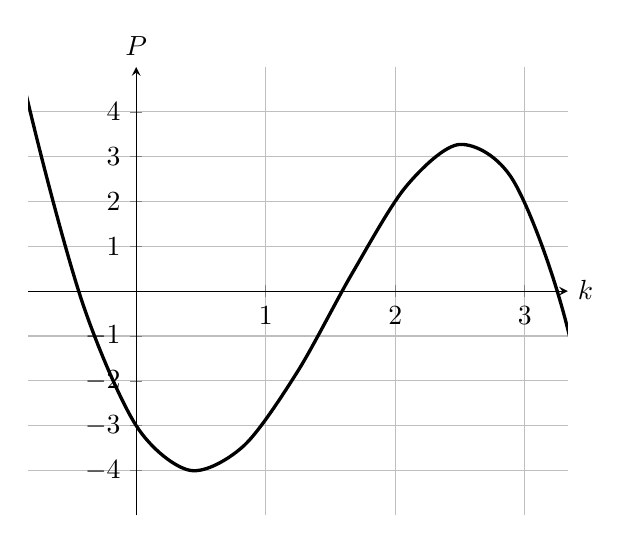
\begin{tikzpicture}
\begin{axis}[
            ymin=-5,
			ymax=5,
            axis lines =center, xlabel=$k$, ylabel=$P$,
              every axis y label/.style={at=(current axis.above origin),anchor=south},
              every axis x label/.style={at=(current axis.right of origin),anchor=west},
            domain=-5:5,
            grid = major,
            xtick={-4,...,4},
            ytick={-4,...,4},
          ]
          \addplot [very thick, smooth] {1 + (3.5 + x)*(-0.5714285714285714 + (-3.5 + x)*(0.16326530612244897 + (-0.3327149041434756 + (-0.20522334808049095 + 0.04019472590901159*(-3 + x))*(-2 + x))*x))};
        \end{axis}
\end{tikzpicture}
\]
\begin{multiple-choice}
\choice[correct]{Yes.}
\choice{No.}
\end{multiple-choice}
\begin{solution}
\begin{hint}
For each input, how many outputs are there?
\end{hint}
\end{solution}
Use the plot to compute $P(2)$
\begin{solution}
\begin{hint}
To start, find $2$ on the horizontal axis. 
\end{hint}
\begin{hint}
Now from this position, move up or down until you reach the curve. The value of $P(2)$ is the height of the curve at the point $k=2$.
\end{hint}
The value of $P(2)$ is \answer{$2$}.
\end{solution}
\end{question}


\begin{question}
In the plot below, is $R$ a function of $n$?
\[
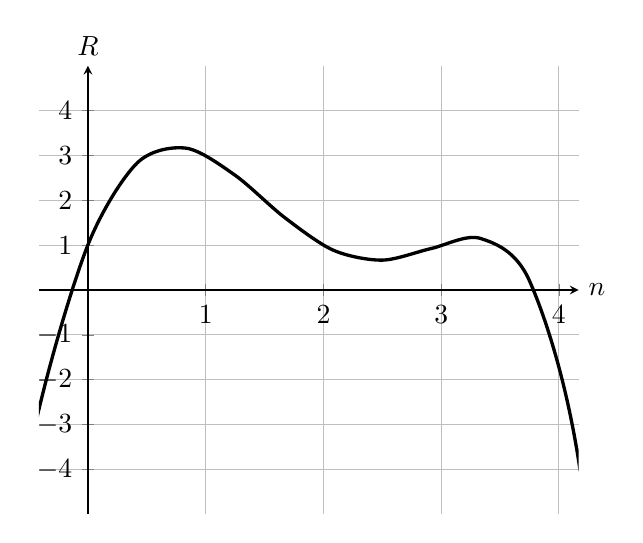
\begin{tikzpicture}
\begin{axis}[
            ymin=-5,
			ymax=5,
            axis lines =center, xlabel=$n$, ylabel=$R$,
              every axis y label/.style={at=(current axis.above origin),anchor=south},
              every axis x label/.style={at=(current axis.right of origin),anchor=west},
            domain=-5:5,
            grid = major,
            xtick={-4,...,4},
            ytick={-4,...,4},
          ]
          \addplot [very thick, smooth] {4 + (-0.42857142857142855 + (-0.05952380952380952 + (0.09163059163059163 + (-0.041447441447441453 - 0.08955488955488956*(-3 + x))*(-2 + x))*(-0.5 + x))*(-3.5 + x))*(3.5 + x)};
        \end{axis}
\end{tikzpicture}
\]
\begin{multiple-choice}
\choice[correct]{Yes.}
\choice{No.}
\end{multiple-choice}
\begin{solution}
\begin{hint}
For each input, how many outputs are there?
\end{hint}
\end{solution}
Use the plot to compute $R(3)$
\begin{solution}
\begin{hint}
To start, find $3$ on the horizontal axis. 
\end{hint}
\begin{hint}
Now from this position, move up or down until you reach the curve. The value of $R(3)$ is the height of the curve at the point $n=3$.
\end{hint}
The value of $R(3)$ is \answer{$1$}.
\end{solution}
\end{question}

\begin{question}
In the plot below, is $b$ a function of $w$?
\[
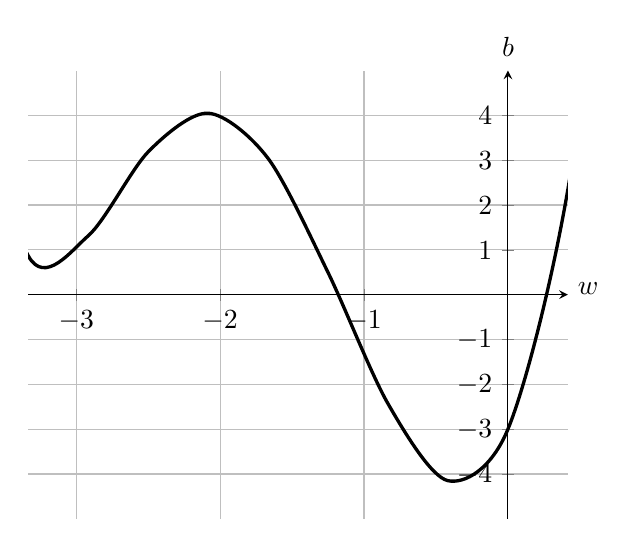
\begin{tikzpicture}
\begin{axis}[
            ymin=-5,
			ymax=5,
            axis lines =center, xlabel=$w$, ylabel=$b$,
              every axis y label/.style={at=(current axis.above origin),anchor=south},
              every axis x label/.style={at=(current axis.right of origin),anchor=west},
            domain=-5:5,
            grid = major,
            xtick={-4,...,4},
            ytick={-4,...,4},
          ]
          \addplot [very thick, smooth] {2 + (3.5 + x)*(0.2857142857142857 + (-3.5 + x)*(0.489795918367347 + x*(0.34013605442176864 + (-0.5850340136054422 - 0.25117739403453676*(-0.5 + x))*(2 + x))))};
        \end{axis}
\end{tikzpicture}
\]
\begin{multiple-choice}
\choice[correct]{Yes.}
\choice{No.}
\end{multiple-choice}
\begin{solution}
\begin{hint}
For each input, how many outputs are there?
\end{hint}
\end{solution}
Use the plot to compute $b(-2)$
\begin{solution}
\begin{hint}
To start, find $-2$ on the horizontal axis. 
\end{hint}
\begin{hint}
Now from this position, move up or down until you reach the curve. The value of $b(-2)$ is the height of the curve at the point $w=-2$.
\end{hint}
The value of $b(-2)$ is \answer{$4$}.
\end{solution}
\end{question}
\end{shuffle}






%%%%%%%%%%%%%%%%%%%%%%%%%%%%%%%%%%%%%%%%%%%%%%%%%%%%%%%%%%%%
%%%%%%%%%%%%%%%%%%%%%%%%%%%%%%%%%%%%%%%%%%%%%%%%%%%%%%%%%%%%
%% Problem
%%%%%%%%%%%%%%%%%%%%%%%%%%%%%%%%%%%%%%%%%%%%%%%%%%%%%%%%%%%%
%%%%%%%%%%%%%%%%%%%%%%%%%%%%%%%%%%%%%%%%%%%%%%%%%%%%%%%%%%%%


\begin{question} 
Suppose you are standing on a bridge that is 60 meters above
sea-level. You toss a ball up into the air with an initial velocity of
30 meters per second.  If $t$ is the time (in seconds) after we toss
the ball, then the height at time $t$ is approximately $f(t) = -5 t^2
+30t+60$. What does $f(2)$ mean in our context?
\begin{solution}
\begin{hint}
We want an answer in the context of the problem. 
\end{hint}
\answer[free-response]{The value $f(2)$ is the height of the ball after $2$ seconds.}
\end{solution}
Now suppose $t$ is such that $f(t) = 100$. What does this mean in our
context?
\begin{solution}
\begin{hint}
We want an answer in the context of the problem. 
\end{hint}
\answer[free-response]{These value of $t$ are the times when the ball is at 100 meters above sea level.}
\end{solution}
Finally, if $h$ is a small positive value what is the meaning of
$f(t+h)$? How does this compare to the meaning of $f(t)+h$?
\begin{solution}
\begin{hint}
We want an answer in the context of the problem. 
\end{hint}
\answer[free-response]{The value $f(t+h)$ gives the height of the ball
  slightly after time $t$. On the other hand, the value $f(t)+h$ gives
  a height just higher than the ball at time $t$.}
\end{solution}
\end{question}


